\section{Modélisation conceptuelle}\label{sec:concept}
% \e{}
% On divise notre problème de modélisation en axes 
% comme il n'existe pas UNE prod.av, on propose des briques représentant des situations typiques paramétrables pour s'ajuster à un usage particulier
% on présente le concept principal, la structure ontologique, les articulations avec le reste de l'ontologie, et un exemple d'utilisation

Comme nous l'avons vu en section \ref{sec:metier}, la production audiovisuelle suit une structure générale qui peut être amenée à changer dans le cadre de productions collaboratives mobilisant des objets existants (\ref{sec:rechaine}) ou bien en fonction du type de production (\ref{sec:strat-desc}).
Ainsi, il apparaît que \gui{\pc{la} production audiovisuelle} n'existent pas, mais recouvrent un ensemble de pratiques et d'usages.
Néanmoins, il existe une tradition de travail et d'organisation de la production en projet, lui-même décomposé en grandes étapes (pré-production, production, post-production) et articulés autour de rôles phares (réalisateur, acteur, chef-opérateur, preneur de son etc.) dont les responsabilités sont, là encore, relativement définies, mais sujettes aux changements suivant la nature de la production, de l'organisation, de traditions nationales etc.

Notre modélisation vise donc à fournir des briques de bases pour représenter l'organisation d'un projet de production.
En suivant la synthèse de scénario de la section \ref{sec:scenar-apps}, cela correspond à l'étape (2) de \g{Planification} qui sera susceptible d'être modifié tout au long de la chaîne, suivant les péripéties de son déroulement.
Cette approche générique permet à chacun de définir sa propre hiérarchie de tâches et de distribuer finement les responsabilités entre les différents contributeurs du projet.


\subsection{Axes de modélisation}
Notre travail de modélisation se heurte à deux verrous scientifiques, identifiés en section \ref{sec:scien} puis développé dans les chapitre \ref{chap:omod} et \ref{chap:mav}, que nous reformulons en : 


\begin{problemes}{LightGoldenrodYellow}
\begin{liste}
 	\item[(\g{$\alpha$})] \g{l'articulation de plusieurs ensembles de connaissances} [\e{$\chi_1$ : autonomie}, \e{$\chi_2$ : réutilisabilité}]. 
 	On distingue ainsi deux ensembles de connaissances : 
 	% à quoi servent-ils ?
 	\begin{listeni} 
 		\item[($\alpha_1$)] l'organisation du \e{processus de production audiovisuelle}, qui décrit la répartition des tâches et  les capacités des \e{contributeurs}.
 		Cet ensemble permet d'associer les connaissances fabriquées par les contributeurs aux documents et de faciliter leur implication et les échanges de connaissances.
 		
 		\item[($\alpha_2$)] l'organisation du \e{document audiovisuel}, c'est-à-dire sa structure documentaire, le \e{matériel audiovisuel} qu'on y attache et une description de leur fabrication (l'\e{écriture filmique} détaillée dans le script).
 		Cet ensemble permet de faciliter la recherche, la gestion et donc la réutilisation des fragments audiovisuels.
 	\end{listeni}

 	\item[(\g{$\alpha$})] et \g{une pro(duction/con)sommation progressive et contributive de ces connaissances} [\e{$\delta_1$: multi-jargon}, \e{$\delta_2$ : documentation}, \e{$\delta_3$ : évolution, gestion}].
 	Il s'agit ici du problème de l'évolution et du partage des connaissances liées à un document/fragment audiovisuel tout au long de son ou de ses cycle(s) de vie. 
 	On distingue deux écueils nouveaux suite à l'ouverture de la chaîne à des pratiques de réutilisation : la \e{progressivité de la description}, et la nécesssité de la rendre compréhensible malgré l'\e{hétérogénéité des contributeurs} : 
 	\begin{listeni}
 		\item[($\beta_1$)] \e{les connaissances sur les document/fragments audiovisuels évoluent et s'ajustent au contexte de production ou de réutilisation}.
 		Les connaissances fabriquées en début de chaîne de production prescrivent un résultat attendu, or de nombeux éléments sont susceptibles d'être modifiés ou précisés par la suite.
 		Il faut donc ajuster les connaissances prescriptives à la réalité des opérations, afin de décrire les résultats effectifs (et non plus l'attendu).
 		Cet écueil apparent est en réalité une opportunité, car la fabrication des descriptions peut alors s'appuyer sur les connaissances prescriptives et les vérifier. 
		De plus, la réutilisation d'un fragment/document audiovisuel dans un nouveau contexte n'implique pas seulement un transfert de matériels audiovisuels, mais également un transfert des connaissances. % mais est-ce que l'on traite vraiment ce cas ? on gère des ensembles de connaissances qui peuvent évoluer (enrichissement)
		Ce transfert peut nécessiter d'extraire certaines connaissances toujours pertinentes et de les associer à celles du nouveau contexte d'utilisation, ou bien de les intégrer à une conceptualisation propre à ce contexte (spécialisation ou bien extension).
		% Cette évolution est rendue possible par 

		\item[($\beta_2$)] \e{adapter la forme d'expression des connaissances en fonction de l'implication du contributeur dans la chaîne de production et de ses capacités.}
 		Le problème de l'accès aux connaissances est traité par la composition d'une vue contextuelle et spécifique à chaque contributeur de la chaîne, ou chaque groupe de contributeurs.
 		Toute connaissance exprimée à travers le modèle doit pouvoir être caractérisée suivant les codes d'écritures utilisés, eux-mêmes reliées aux capacités des contributeurs.
		Il est alors possible d'effectuer une double sélection ; les connaissances pertinentes suivant l'implication dans la chaîne (en utilisant la description du processus de production); les formes d'expression facilitant leur compréhension (à partir d'une description des capacités des contributeurs).
		% Cette adaptation est rendue possible par le couplage entre conceptualisation, terminologie et documentation.
 	\end{listeni}
\end{liste}
\end{problemes}

% (\ref{sec:cdc-av}). 



% Par ailleurs, les objectifs métiers de réutilisation ouvre la chaîne de production à de nouveaux contributeurs, dont les niveaux de compétences et de compréhension sont variables (\ref{sec:cdcf}). 
% Les connaissances liées à la production doivent être rendues accessibles à toutes les contributeurs de la chaîne, de même qu'ils doivent contribuer à la fabrication de ces connaissances, tout autant que la fabrication d'objets audiovisuels ou de documents métiers. 

% L'approche que nous avons suivi se positionne sur deux axes de modélisation : 
% \begin{liste}
% 	\item[\g{$\alpha$}] articuler une modélisation conceptuelle aux problèmes de partage et de construction de connaissances communes d'une chaîne de production audiovisuelle ouverte et hétérogène. 
% 	Nous traitons dans cet axe les problèmes définis dans le chapitre \ref{chap:omod} sur la nécessité de construire des terminologies multi-jargon [\g{A1}], d'enrichir une conceptualisation avec de la documentation [\g{A2}], et de gérer l'évolution des unes et des autres de manière indépendantes [\g{A3}].



[Relations transitives pour faciliter l'inférence (SKOS) ; distinction entre objet réel (production) et fictif (diégèse) (DMS-1).]


\subsection{Situations typiques des productions audiovisuelles}
Notre modélisation peut se décomposer en situations typiques qui se retrouvent dans tous les types de productions audiovisuelles.
Nous présentons ces situations en rapport avec les axes de modélisations que nous avons défini :
\begin{listeni}
	\item[($\alpha_1$)] l'organisation du \g{processus de production} et du travail de ses \g{contributeurs} : 
	\begin{liste}
		\item la division d'un projet de production en sous-tâches et la spécification du résultat attendu ainsi que des moyens fournis pour les remplir.

		\item l'assignation des tâches d'un projet à des contributeurs, ce qui leur confère un rôle, des droits et des responsabilités.
	\end{liste}

	\item[($\alpha_2$)] l'articulation d'un \g{document audiovisuel} et de ses différentes composantes, avec leurs descriptions : 
	\begin{liste}
		\item la structure documentaire qui suit des règles de composition de fragments.
		\item la segmentation du matériel audiovisuel.
		\item la gestion des fichiers qui encapsulent le matériel audio-visuel et ces différentes pistes.
		\item la description par l'écriture filmique, et ses références à des éléments fictifs ou réels.
	\end{liste}


	\item[($\beta_1$)] le déroulement de la production a pour conséquence de faire \g{évoluer nos connaissances} sur l'organisation du processus de production et l'articulation du document audiovisuel : 
	\begin{liste}
		\item les pratiques de réutilisation de fragments documentaires.
		\item l'évolution de la description d'un document audiovisuel.
		\item l'échange de connaissances entre organisations.
	\end{liste}

	\item[($\beta_2$)] l'\g{adaptation des formes d'expressions} aux capacités des contributeurs de la chaîne de production : 
	\begin{liste}
		\item l'attribution de compétences linguistiques et professionnelles aux contributeurs (humains, machines).
		\item la mise en place d'un thésaurus multi-jargon et d'une documentation des concepts.
		\item l'accès personnalisé aux connaissances de la chaîne suivant le contexte (le contributeur, ses capacités, son implication dans la châine).
	\end{liste}

\end{listeni}



%%%%%%%%%%%%%%%%%%%%%%%%%%%%%%%%%%%%%%
\subsubsection{Articulation des composantes d'un document audiovisuel}\label{sec:opus}
La modélisation d'un document audiovisuel numérique implique des composantes distinctes que nous avons étudié en \ref{sec:dav}. 
Ainsi, nous le modélisons par trois composantes autonomes (au sens où elles peuvent être manipulé indépendamment des autres) mais qui s'articulent pour représenter un document et ses fragments. 
La Figure \ref{img:so-cr-dav} présente les principaux concepts et relations qui modélisent un document audiovisuel, dont nous introduisons quelques définitions avant de les détailler par composantes : 
\begin{liste}
	\item la \g{manifestation matérielle}, c'est-à-dire l'enregistrement du matériel audiovisuel en numérique, selon un codage donné.
	La manifestation matérielle d'un objet audiovisuel est représentée dans des fichiers numériques (\con{DigitalResource}), comme des fichiers d'encapsulation de média (\con{MediaWrapper}), ou des portions de ces fichiers que l'on nomme piste (\con{Track}) dans le cas des contenus temporels.

	\item la \g{segmentation du matériel audiovisuel}, c'est-à-dire le matériel sous sa forme temporelle, une fois décodé (rendu perceptible) par une dispositif de lecture. 
	De manière générale, le décodage d'une manifestation matérielle produit une forme perceptible (\con{ContentObject}), ce qui dans le cas du matériel audio ou audio-visuel peut être représenté par une forme temporelle (\con{TemporalObject}).
	Pour caractériser ces formes temporelles, on considère deux spécialisations, le \con{Segment} qui représente une séquence, et la \con{Segmentation} qui représente une collection ordonnée d'objets temporels (\con{TemporalObject}).
	Un point important à noter est qu'une même forme temporelle peut être construites à partir de différentes \con{DigitalResource}, qu'il s'agisse de copies ou bien de variantes d'encodage. 
	
	\item la \g{forme sémiotique}, celle qui est interprétable par un lecteur, et qui donne à voir la structure du document et ses règles de composition.
	De manière générale, cette forme sémiotique représente le résultat d'un travail artistique, intellectuel, technique (\con{Opus}).
	Nous distinguons en particulier l'oeuvre dans son ensemble (\con{MediaAsset}) qui représente un document à part, et les fragments qui le composent (\con{EditorialObject}).
	Il nous faut remarquer que notre modélisation d'un document audiovisuel repose sur les deux précédentes composantes (\con{DigitalResource} et \con{ContentObject}) qui correspondent à la fabrication du matériel audiovisuel et à son montage et ses retouches pendant la post-production.
	Cette dernière composante enrichit cette modélisation classique d'une dimension documentaire et éditoriale, et permet de les articuler afin de faciliter la création de variantes ou la réutilisation de fragments pour de nouveaux documents (voir notre caractérisation de ces pratiques, section \ref{sec:reuse}).
	De plus, en se détachant du matériel audiovisuel, cette composante nous permet de capturer des connaissances sur la structure du document avant même sa production, et d'y attacher des connaissances (\con{Annotation}).
\end{liste}

\begin{figure}[ht!]
\centering
\includegraphics[width=0.95\textwidth]{./images/SO-CR-DAV-v2.png}
\caption{Principaux concepts et relations pour modéliser les composants d'un document audiovisuel}
\label{img:so-cr-dav}
\end{figure}

\subsubsection*{Manifestation matérielle}
\begin{cadrecol}{LightGoldenrodYellow}
Une \con{DigitalResource} représente une séquence de bits, comme un fichier ou une partie d'un fichier. 
L'adresse de la ressource effective est donnée par la propriété \rel{source}. 
\end{cadrecol}
D'autres relations définissent le concept de ressource numérique :
\begin{liste}
	\item une \con{DigitalResource} peut également être la représentation (manifestation) numérique des autres types d'entités par la relation \rel{isAManifestationOf}/\rel{hasManifestation}, et plus spécifiquement représenter une illustration (graphique, textuelle, sonore etc.) d'une entité par la relation \rel{illustrates}/\rel{isIllustratedBy}.
	Par exemple, un \con{Program} a pour manifestation un \con{AudiovisualMedia}, une \con{Segmentation} a pour manifestation un fichier EDL, un \con{Segment} sera représenté par une portion de fichier EDL etc.
	D'autres \con{Entity} peuvent avoir des manifestations, par exemple lorsqu'elles sont représentés en-dehors de notre modélisation.\\
	
	\item une \con{DigitalResource} peut également avoir des copies (\rel{hasCopy}), identiques en tous points, sauf l'adresse. 
	\item il est possible de spécifier le support de stockage (\con{Medium}) utilisé pour enregistrer la \con{DigitalResource} (\rel{isRecordedOn}).\\
	
	\item une relation spécifique (\rel{conformsTo}) permet d'indiquer l'encodage des caractères et le format de fichier utilisé (\con{SyntaxEncodingScheme}).
	\item d'autres informations, comme le vocabulaire ou bien le système d'écriture utilisé (\con{Notation}) sont indiqués par la relation \rel{isMemberOf}/\rel{hasMember}.
\end{liste}



\begin{figure}[ht!]
\centering
\includegraphics[width=0.95\textwidth]{./images/SO-DR-v1.png}
\caption{Principaux concepts et relations pour modéliser les manifestations matérielles numériques}
\label{img:so-dr}
\end{figure}


Au niveau de la structure ontologique, la Figure \ref{img:so-dr} montre qu'une \con{DigitalResource} se spécialise soit en \con{MediaWrapper}, soit en \con{Track} selon que la séquence de bits constitue un fichier ou une portion de fichier.
Par la suite, ces deux concepts se spécialisent en fonction du critère différentiel suivant ; la nature du matériel qui est représenté. 
Pour les \con{Track}s, on distingue la version audio (\con{AudioTrack}), vidéo (\con{VideoTrack}) et celles des sous-titres (\con{SubtitlesTrack}).
D'autres types de pistes peuvent être ajoutés par la suite, par exemple pour identifier la piste télétexte etc.
\begin{cadrecol}{LightGoldenrodYellow}
\con{MediaWrapper} représente une manifestation numérique et fournit les informations nécessaires à sa lecture.
\end{cadrecol}
\begin{cadrecol}{LightGoldenrodYellow}
Une \con{Track} est une manifestation matérielle qui contient un contenu temporel. 
La lecture de ce contenu se fait selon une vitesse donnée et fixe, ce qui permet de synchroniser plusieurs \con{Track}s de nature différentes pour former un contenu multi-modal. 
Par exemple, un fichier .mkv contient une piste de sous-titre pour un documentaire. 
Les sous-titres sont formés d'une série de mots indexés par des codes temporels (timecode), qui déterminent quand les mots doivent être affichés. 
\end{cadrecol}

Pour les \con{MediaWrapper}, on distingue trois concepts enfants : 
\begin{liste}
	\item \con{GraphicalMedia} représente du contenu graphique, c'est-à-dire des images (\con{ImageMedia}) ou du texte (\con{TextMedia}). 
	Par exemple, un fichier PDF d'un livre, ou bien une photo en format .jpg.
	\item \con{TemporalMedia} représente du contenu temporel avec une vitesse de lecture et une durée fixe, comme une vidéo (\con{AudiovisualMedia}) ou bien une chanson (\con{AudioMedia}).
	\item \con{InteractiveMedia} représente des contenus interactifs et dynamique, et dont la durée de lecture n'est pas fixé a priori, mais varie en fonction de l'interaction avec le lecteur.
	Il peut s'agir par exemple d'un programme ou bien d'un jeux vidéo. 
\end{liste}


\subsubsection*{Segmentation du matériel audiovisuel}
\begin{cadrecol}{LightGoldenrodYellow}
Un \con{ContentObject} représente le résultat du décodage (ou de la lecture) d'une manifestation matérielle, c'est-à-dire une forme perceptible de la manifestation.
\end{cadrecol}


Cette définition peut être spécialisée suivant le type de média qui est produit par la lecture de la manifestation matérielle ; un \con{TemporalObject} pour les formes temporelles construites à partir d'un \con{TemporalMedia} ; un \con{GraphicalObject} pour les formes graphiques construites à partir d'un \con{ImageMedia} ; un \con{TextualObject} pour les formes composées de texte construites à partir d'un \con{TextMedia}, voir Figure \ref{img:so-content}.
Pour chacun de ces formes, on peut distinguer ensuite deux concepts enfants :
\begin{listeni} 
	\item le premier représentant une \e{sélection} sur la forme. 
	Dans le cas d'une forme temporelle, on utilise le code temporel (timecode) pour effectuer des sélections (\con{Segment}) sur une source (\con{TemporalMedia}, \con{TemporalObject}, \con{Track}) par la relation \rel{hasSource}. 
	Les attributs \rel{TCin} et \rel{TCout} permettent d'indiquer le début et la fin de la sélection en utilisant la source comme référence.
	
	\item l'autre représentant un \e{assemblage} de sélections. 
	Une \con{Segmentation} représente une collection (non-ordonnée) de \con{TemporalObject}, relié par la relation \rel{assembles}. 
	Cela peut être une collection de \con{Segment}s (ceux qui sont utilisées pour construire le montage) ; un assemblage de \con{Segmentation} existantes (par exemple, l'insertion d'une interview dans un documentaire) ; un assemblage composite de \con{Segment}s et de \con{Segmentation}.
	Il est à noter qu'une \con{Segmentation} ne représente pas finement le montage, comme des EDL, mais simplement une liste de séquences. Une \con{Segmentation} peut être relié à l'EDL correspondante par la relation \rel{hasManifestation}.
\end{listeni}

\begin{figure}[ht!]
\centering
\includegraphics[width=0.75\textwidth]{./images/SO-ContentObject-v1.png}
\caption{Extrait de la structure ontologique qui modélise la segmentation du matériel audiovisuel}
\label{img:so-content}
\end{figure}

\paragraph{Sélectionner une portion de ressource}
Il est à remarquer que ces concepts de sélection (\con{Segment}) fonctionnent à partir d'un repère (c'est-à-dire de dimensions) ou bien d'un langage de sélection (comme CSS pour le HTML) qui permettent d'identifier des portions de contenu.
Dans le cas du texte, les caractères peuvent servir de métrique pour identifier les portions de contenu à sélectionner. 
De manière similaire, une image ou un objet 3D utilisent un repère (x,y,z) ou autres pour situer les formes construites sur l'espace de travail.
Dans le cas de média interactif, ce problème est moins évident à traiter et doit se gérer au cas par cas, suivant le format utilisé. 
Nous n'avons pas poussé notre modélisation sur ces aspects, car notre approche n'a pas besoin de détailler ces aspects, et que par ailleurs MPEG-7 propose des solutions éprouvées.

\paragraph{Lister les éléments utilisés dans un assemblage}
Concernant la notion d'assemblage de matériel audiovisuel (\con{Segmentation}), notre modélisation se limite à lister les \con{Segment}s utilisés, mais pourrait être étendu pour gérer la notion d'ordre.
Cependant, de nombreux formats de représentation du montage (Edit Decision List) existent par ailleurs, largement plus expressifs et déjà intégrés dans certaines applications. 
Ainsi, notre approche permet de faire une liste des éléments utilisées et laissent la représentation fine du montage à ces formats externes, que l'on peut raccrocher à notre modèle par la relation \rel{hasManifestation}.


\subsubsection*{Structure documentaire}
\begin{cadrecol}{LightGoldenrodYellow}
Un \con{Opus} est une forme documentaire qui résulte de l'articulation d'un travail artistique, intellectuel et technique.
De ce fait, le concept \con{Opus} est directement relié avec les concepts de \con{DigitalResource} (relation \rel{hasManifestation}) et de \con{ContentObject} (relation \rel{hasRealisation}) ainsi qu'avec d'autres \con{Opus} qui définissent sa structure documentaire (relation \rel{composedOf}).
Dans le cadre d'une modélisation dynamique suivant un processus de production, l'\con{Opus} est le concept sur lequel on peut rattacher des connaissances a priori sur le document à fabriquer (relation \rel{hasPrescription}) ainsi que les connaissances sur ce qui a été effectivement fabriqué (relation \rel{hasDescription}).
\end{cadrecol}

\begin{figure}[htb!]
\centering
\includegraphics[width=0.95\textwidth]{./images/SO-Opus-v1.png}
\caption{Extrait de la structure ontologique qui modélise les structures documentaires}
\label{img:so-opus}
\end{figure}

La Figure \ref{img:so-opus} présente les spécialisations du concept d'\con{Opus}.
Le premier critère différencie les documents entiers, que l'on estime prêt à être publié (\con{MediaAsset}), des fragments documentaires, qui servent à de briques pour composer les documents (\con{EditorialObject}).
Le concept de \con{Program} représente les documents audiovisuels fabriqués par la production télévisuelle. 
Il s'agit d'un type de document ajusté aux contraintes et spécificités d'une forme de distribution. 
Notre modélisation se limite aux documents audiovisuels, mais il serait possible à ce niveau de définir d'autres types de formes documentaires pour représenter par exemple les documents textuels de la chaîne de production.
Pour cela, il faudrait introduire une typologie des documents semblables à celles proposées pour les \con{DigitalResource}s.
Ensuite, pour chaque type de documents, on peut encore définir des genres et sous-genres, par exemple selon une taxinomie développée par une organisation, comme dans le case de \cite[Annexe B]{Troncy2004}.
Dans notre cas, nous avons donné l'exemple d'un \con{Drama} et d'un \con{Magazine} d'information, qui renvoit alors à des grammaires de compositions propres. 
Cependant, comme nous le précise \cite[\S3.6]{Gaillard2008}, la notion de genre n'est pas forcément à prendre comme l'instanciation d'une \gui{structure normative figée}, mais peut s'envisager davantage comme des règles évolutives de fabrication, qui servent tant à guider la production que la lecture des documents.
Notre approche aborde ces questions de manière minimale, en proposant la possibilité de définir des règles de composition (contraignantes ou non) des \con{MediaAsset} par des \con{EditorialObject}s.
Par défaut, un \con{Drama} est composé d'\con{EditorialObject}s, dont des \con{Scene}. 
De même, un \con{Magazine} est composé d'\con{EditorialObject}s, dont des \con{Subject}, c'est-à-dire de courts reportages que l'on nomme Sujet dans le milieu de la télévision. 

\paragraph{Décomposition en plans et sous-plans}
Ainsi, les spécialisations d'\con{EditorialObject} permettent de définir des unités documentaires, et en particulier les unités de bases que nous avons identifiées ; le \con{Shot} et le \con{Subshot}.
Le \con{Shot} est une série d'images continues ou non coupée par une transition.
La notion de \con{Subshot} correspond aux portions de \con{Shot} où le mouvement de la caméra est ininterrompu ou que le cadrage est constant.
Cela permet de diviser le plan en sous-plans avec une description du mouvement de caméra fixe.
Ainsi, cela permet de décrire des plans complexes où se succèdent différents cadrages. 
Par exemple, une séquencete qui comprend un premier mouvement de caméra (suivant un personnage qui marche) puis un zoom (sur la main du personnage) sera représenté comme un plan (\con{Shot}), comprenant deux sous-plans (\con{Subshot}), l'un pour le travelling, l'autre pour le zoom. 

\paragraph{Prise de vue et sélection de plan}
Au moment du tournage on parle plus de prise de vue que de plan, car cela correspond à la série d'images capturée par une caméra entre le moment où l'enregistrement est lancé et celui où il est arrêté.
Pendant le derushing, on sélectionne juste la portion de la prise de vue qui est utile (voir section \ref{sec:preprod} pour un rappel sur le déroulement de la chaîne de production).
La distinction entre les résultats de ces deux étapes est représenté par les concepts d'\con{AudiovisualMedia} (qui modélise la prise de vue enregistré par le caméraman) et de \con{Segment} (qui modélise la sélection d'une séquence par le derusheur), relié par une relation \rel{hasSource}.
Lorsque plusieurs prises du même plan ont été tournées, on se retrouve alors avec plusieurs \con{Segment}s qu'il faut ensuite relier au plan (\con{Shot} qui est un \con{EditorialObject}).
Dans ce cas, le lien entre ces prises et le plan est représenté par des relations \rel{hasRealisation} indiquant que les \con{Segment} sont des expressions de la forme documentaire \con{Shot}.
Pour être plus précis et distinguer entre les des versions alternatives d'un même plan, et la version finalement retenue, on spécialise la relation \rel{hasRealisation} en \rel{hasCandidateRealisation} (pour les versions alternatives) et \rel{hasFinalRealisation} (qui indique la version choisie dans le montage final).
Il est à remarquer que les versions alternatives pointent vers les fichiers créés au moment du tournage, alors que la version finale pointe par le fichier qui résulte du montage. 
Si la modélisation des versions de travail et de la version finale du document est séparée à ce niveau là, le fait de les rattacher aux mêmes \con{Opus} et d'utiliser ces relations spécifiques permet d'expliciter leur statut tout en partageant leur description (\con{Annotation}). 


\paragraph{Attacher des connaissances au document audiovisuel}
Notre modélisation du document audiovisuel permet d'attacher des connaissances au cours de la production du document audiovisuel.
Le vocabulaire de l'écriture filmique est représenté par des \con{Annotation}s, que nous définirons plus précisément dans la section \ref{sec:annotation}. 
Avant la fabrication du matériel audiovisuel, les \con{Annotation}s, reliées à la structure du document (\con{Opus}) par la relation \rel{hasPrescription}, représentent le script et servent de guide de tournage, notamment dans le cadre de production collaborative amateur-professionnel.
Après le tournage, les \con{Annotation}s peuvent être utilisé pour décrire (relation \rel{describes}) des séquences de matériel effectivement fabriqué (plus précisément, les \con{Segment}s qui sélectionnent des bouts d'\con{AudiovisualMedia} ou de \con{VideoTrack}).
Il faut noter que cette description est indépendante de la prescription, car il faut pouvoir rendre compte des plans non prévus dans le plan de tournage, comme les \gui{plans de coupe} qui servent à faire des transitions ou à introduire un plan intérieur en présentant d'abord l'extérieur d'un bâtiment.
Néanmoins, cette description peut être réalisé par analyse automatique ou manuelle du signal, et par comparaison avec les connaissances prescriptives si besoin.
Les connaissances attachées sur le matériel utilisé dans le montage final peuvent être ensuite associées au document ou à ses fragments (\con{Opus}) par la relation \rel{hasDescription}.



% Évolution de la modélisation : on distingue trois phases
% - avant la fabrication : connaissances prescriptives associées à la structure documentaire pour préparer le tournage. [Annotations --hasPrescription-> Opus]
% - après la fabrication : connaissances descriptives construites par analyse automatique/manuelle, par comparaison avec les co.prescritives pour préparer la sélection du contenu le plus pertinent. [Annotations --describes-> AVMedia]  
% - après le dérushing : [EditorialObject --hasCandidateRealization-> Segment --hasSource-> AVMedia + MA-->hasCandidateRealization-> Segmentation]
% - après le montage : [MediaAsset --hasFinalRealization-> Segmentation --assembles--> Segment --hasSource--> AVMedia + Opus --hasDescription-> Annotations --describes--> AVMedia, ceux qui sont utilisées dans la FinalRealization]
 
\begin{figure}[htb!]
\centering
\includegraphics[width=0.75\textwidth]{./images/UC-evolution-v3a.png}
\caption{Exemple de modélisation documentaire dans les premières étapes de la production audiovisuelle (de la préproduction jusqu'aux premiers montages)}
\label{img:uc-evo1}
\end{figure}

\paragraph{Évolution de la modélisation pendant la production}
Notre modélisation des différentes composantes du document audiovisuel permet également de suivre l'évolution de la chaîne de production. 
Ainsi, les résultats de plusieurs étapes de la chaîne sont représentés dans notre modèle, ce qui facilite son suivi et la reprise du travail ou sa délégation à d'autres contributeurs.
Si l'on détaille le scénario d'usage que nous utilisons dans notre mémoire, nous pouvons à quel moment de la chaîne les instances de nos concepts modélisant le document audiovisuel sont construites, voir la Figure \ref{img:uc-evo1} :
\begin{liste}
	\item Pendant la \g{préproduction}, le script permet de définir à la fois la structure documentaire (\con{MediaAsset} et \con{EditorialObject} reliés par des relations \rel{isComposedOf}) et ainsi que les connaissances qui prescrivent la forme de chaque plan (\con{Annotation}, que nous détaillerons plus tard, reliés au plan par une relation \rel{hasPrescription}).
	Dans notre cas, il s'agit d'une \e{interview} d'un metteur en scène contenant plusieurs plans réalisés en intérieur (même si nous n'en montrons qu'un dans la Figure) et qu'il faudra enrichir de \e{plans de coupe} (non décrits) de l'extérieur du lieu culturel où se déroule la représentation.

	\item Au moment du \g{tournage}, du matériel audiovisuel est créé (\con{AudiovisualMedia}). 
	Dans notre cas, il s'agit de deux fichiers vidéo, l'un contenant plusieurs plans de coupe, l'autre avec une seule prise de vue du réalisateur.
	Pour l'instant, ces instances ne sont reliées à aucun autre composant du document audiovisuel.

	\item Lors du \g{derushing}, il est alors question de sélectionner les parties utiles dans les fichies vidéos (\con{Segment} reliés aux \con{AudiovisualMedia} par une relation \rel{hasSource}).
	On peut ainsi identifier à quels plans correspondent les images tournées (les \con{Segment}s sont reliés à des \con{Shot}s par des relations \rel{hasCandidateRealisation}).
	Il se constitue ainsi une chaîne de relations entre des \con{EditorialObject}s, qui représentent une forme documentaire, et des \con{Segment}s(\rel{hasRealisation}, qui représentent des séquences de matériel audiovisuel, et des \con{AudiovisualMedia} (relation \rel{hasSource}, qui représentent les enregistrements du matériel audiovisisuel.

	\item Au cours du \g{montage}, des \con{Segmentation}s sont construites pour chaque version du montage, listant par la relation \rel{assembles} les \con{Segment}s qui sont utilisées. 
	Ces \con{Segmentation}s correspondent à l'expression (relation \rel{hasCandidateRealisation}) d'\con{EditorialObject} de plus haut-niveau que les plans, ou bien à des \con{MediaAsset} entiers.
\end{liste}

\begin{figure}[htb!]
\centering
\includegraphics[width=0.8\textwidth]{./images/UC-evolution-v3b.png}
\caption{Exemple de modélisation documentaire dans les dernières étapes de la production audiovisuelle (montage final et finition)}
\label{img:uc-evo2}
\end{figure}

\begin{liste}
	\item À la fin du \g{montage} une version finale du montage est choisie, ce qui permet de construire une ou plusieurs manifestation(s) du document audiovisuel. 
	La Figure \ref{img:uc-evo2} montre les instances et les relations créés à cette étape dans des couleurs vives, alors que les anciennes sont dans des couleurs atténuées.
	Dans notre modèle, cela correspond à relier le document (\con{MediaAsset}) à une \con{Segmentation} qui est identifié comme la dernière version par la relation \rel{hasFinalRealisation}.
	Cette \con{Segmentation}, renvoit elle-même à des \con{Segment}s qui détaille la position des plans dans l'enregistrement du matériel audiovisuel construit (\con{AudiovisualAsset}). 
	Dans notre cas, on a construit deux manifestations du document de qualité différente, reliés au \con{MediaAsset} par la relation \rel{hasManifestation}.
	Ces deux instances représentent le résultat de l'étape de \g{finition} qui marque la fin de la post-production et permet l'exploitation du document audiovisuel.
	Au niveau des descriptions, il est possible alors de les relier aux nouveaux \con{Segment}s créés ainsi qu'aux \con{EditorialObject}s correspondants.
	En effet, le montage a simplement permis de rassembler du matériel audiovisuel, auparavant dispersé, dans une même fichier vidéo. 
	Il n'y a donc ni de changement au niveau de sa description (\con{Annotation}), ni au niveau de sa structure documentaire (\con{Opus}).
\end{liste}
















%%%%%%%%%%%%%%%%%%%%%%%%%%%%%%%%%%%%%%
\subsubsection{Description par l'écriture filmique}\label{sec:annotation}
\paragraph{Structure ontologique}
\paragraph{Relations avec d'autres concepts}



%%%%%%%%%%%%%%%%%%%%%%%%%%%%%%%%%%%%%%
\subsubsection{Hiérarchie des tâches dans un projet de production}\label{sec:mission}
La définition d'une hiérarchie de tâches repose sur la définition d'une unité de travail représenté par le concept de \con{Mission} : 

\begin{cadrecol}{LightGoldenrodYellow}
Une \con{Mission} représente un ensemble d'actions cohérentes, réalisées de manière intentionnelles afin de mener à bien un processus de production. 
Ces actions peuvent être exécutées par un ou plusieurs contributeurs, réutilisant parfois des objets existants (ressource), et aboutir à la gestion du processus de production (\con{Mission} de gestion ou de validation : \con{Project} et \con{Activity}), ou bien à la fabrication d'un résultat attendu (ou livrable, pour les \con{Mission}s de fabrication : \con{Task}). 
Par exemple, une \con{Mission} de tournage peut être réalisée par un caméraman, ou bien une équipe de tournage et aboutit à la fabrication de matériel audiovisuel.
\end{cadrecol}

 

\paragraph{Structure ontologique} 
La production d'un film requière de nombreux contributeurs et la spécification de nouvelles \con{Mission}s.
Ainsi, on distingue les \con{Mission}s (dites de gestion) qui consistent à en définir d'autres, à suivre leur déroulement et à valider le résultat fabriqué par les \con{Mission}s de fabrication. 
Nous distinguons trois types de \con{Mission} par leur nature et leur importance en terme de durée : 
\begin{liste}
	\item un \con{Project} représente un projet de production, qui renvoit à entité administrative auquelle une organisation transfère des ressources (humaines, financières, équipements etc.) pour accomplir des objectifs. 
	Il s'agit d'une \con{Mission} de gestion qui ne fabrique rien, mais dirige, organise et délégue le travail et les ressources à d'autres \con{Mission}s (\con{Activity} et \con{Task}).
	Par exemple, le \con{Project} Magazine\#48 représente le processus de création de l'épisode 48 d'un programme d'information (résultat), qui consiste à commenter des évènements culturels de l'année dernière (ressource).

	\item une \con{Activity} est une étape ou un jalon d'un projet de production. 
	C'est une \con{Mission} de gestion qui consiste à organiser une séquence de \con{Task}s.
	Par exemple, une \con{Activity} nommée Post-Production peut regrouper toutes les \con{Task}s montage, retouches, effets spéciaux, post-traitements etc.

	\item une \con{Task} est une \con{Mission} opérationnelle qui vise généralement à fabriquer ou manipuler un objet audiovisuel ou des connaissances associées.
	Par exemple, le tournage d'une interview ou bien la transformation du scénario en script de tournage. 
\end{liste}

\begin{figure}[ht!]
\centering
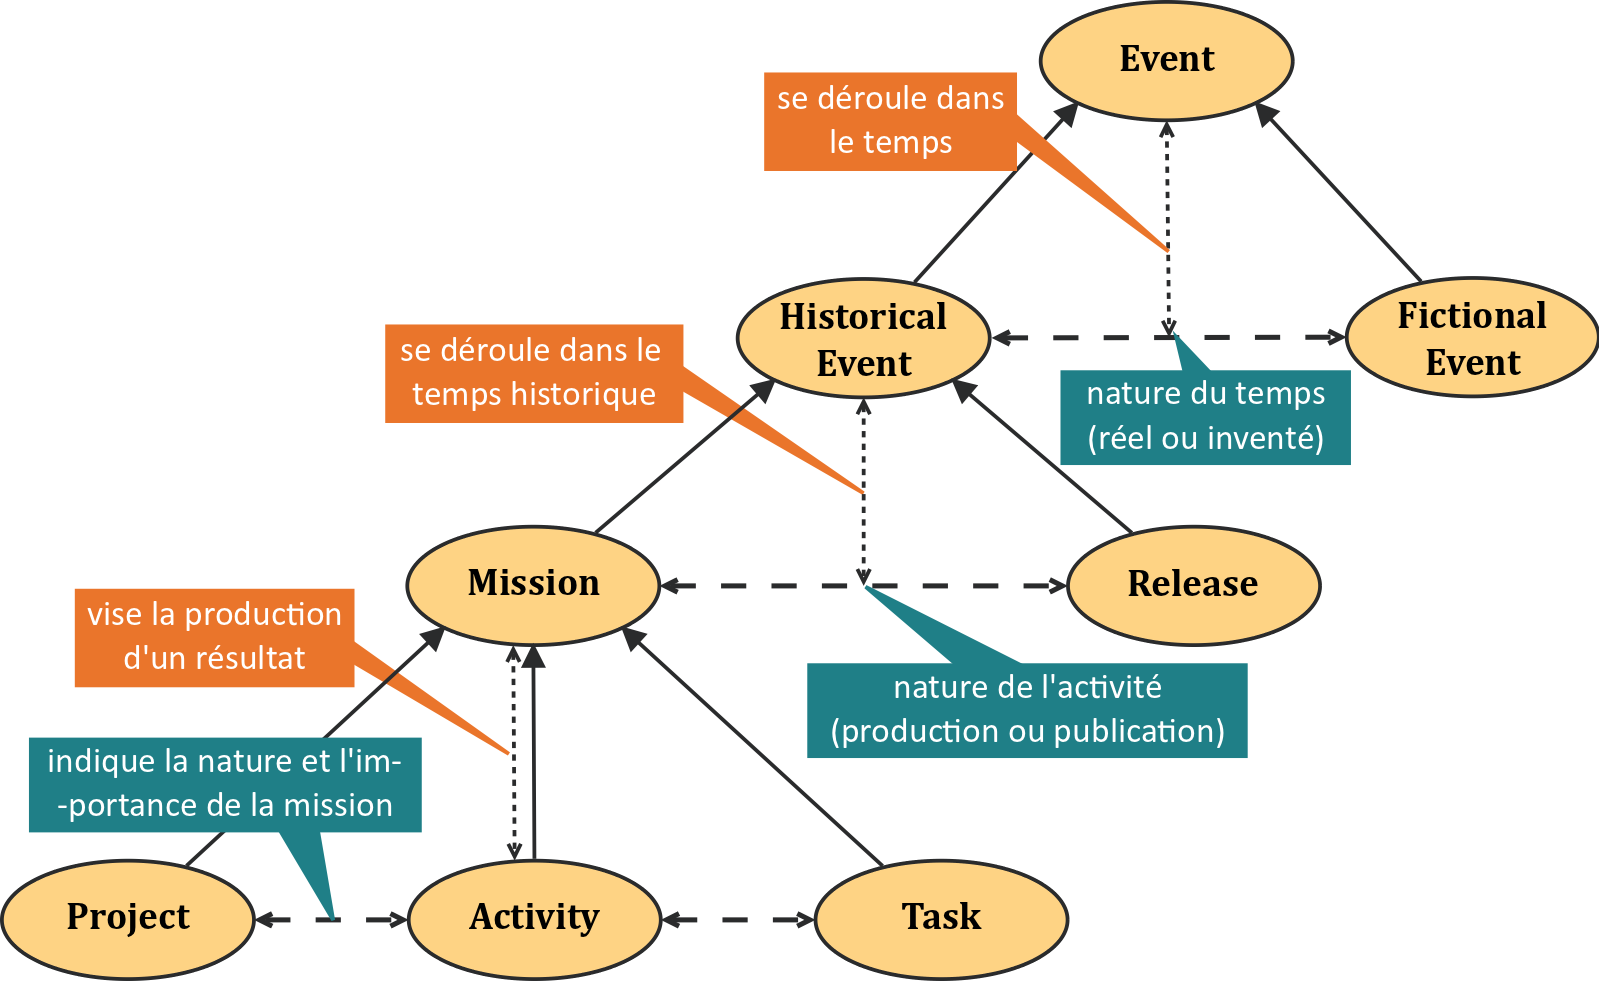
\includegraphics[width=0.95\textwidth]{./images/SO-Event-v1.png}
\caption{Extrait de la structure ontologique qui modélise les évènements et de la hiérarchie des tâches d'un projet de production}
\label{img:so-event}
\end{figure}


La Figure \ref{img:so-event} précise la structure ontologique des évènements et en particulier la hiérarchie des tâches d'un projet de production.
Un point important à noter est que notre modélisation ne distingue pas les objets temporels duratifs et ponctuels, mais laisse libre choix de préciser le moment de début et de fin d'un \con{Event} à travers les propriétés \rel{Start} et \rel{End}.
Au lieu de cela, nous distinguons les évènements réels (\con{HistoricalEvent}) des évènements fictifs (\con{FictionalEvent}), qui sont mis en scène pour être filmé. 
Cette distinction se retrouve dans d'autres parties de notre modélisation et apparaît importante pour distinguer les connaissances liées à la production de celles liées à l'univers filmé (contrairement à la confusion qui existe dans DMS-1, voir \ref{sec:dms-1}).



\paragraph{Relations avec d'autres concepts}
Le concept d'\con{Event} et de \con{Mission} se définissent également par leurs relations avec le reste de notre ontologie, voir la Figure \ref{img:cr-event}. 
Voici les relations qui s'appliquent à tous les évènements : 
\begin{liste}
	\item il est possible de spécifier la participation d'une personne ou d'une organisation (\con{Agent}) à l'évènement (par la relation \rel{hasParticipant}/\rel{isAParticipantOf}).
	Cette relation présente une version simplifiée de notre modélisation de l'implication d'un contributeur dans un projet de production.
	Nous ajoutons également une contrainte de cohérence : dans le cas où il s'agit d'évènement réel, seul des participants réels peuvent être associées à l'évènement (et inversement). 
	Par exemple, Batman ne peut pas participer à une manifestation sur la place de la Bastille, par contre Benjamin Diemert si. 

	\item il est possible de localiser (\con{Location}) l'évènement (par la relation \rel{isLocatedIn}).
	Cette relation en fonctionne que dans un seul sens et ne peut pointer que vers un lieu, qui lui-même est liée à d'autres lieux par des relations méréologiques ou d'autres relations géographiques.
	Nous ajoutons également une contrainte de cohérence : un évènement réel ne peut se situer dans un lieu fictif.

	\item Les évènements peuvent également être le sujet d'une oeuvre (\con{Opus}) grâce à la relation \rel{isATopicOf}. 
\end{liste}


\begin{figure}[ht!]
\centering
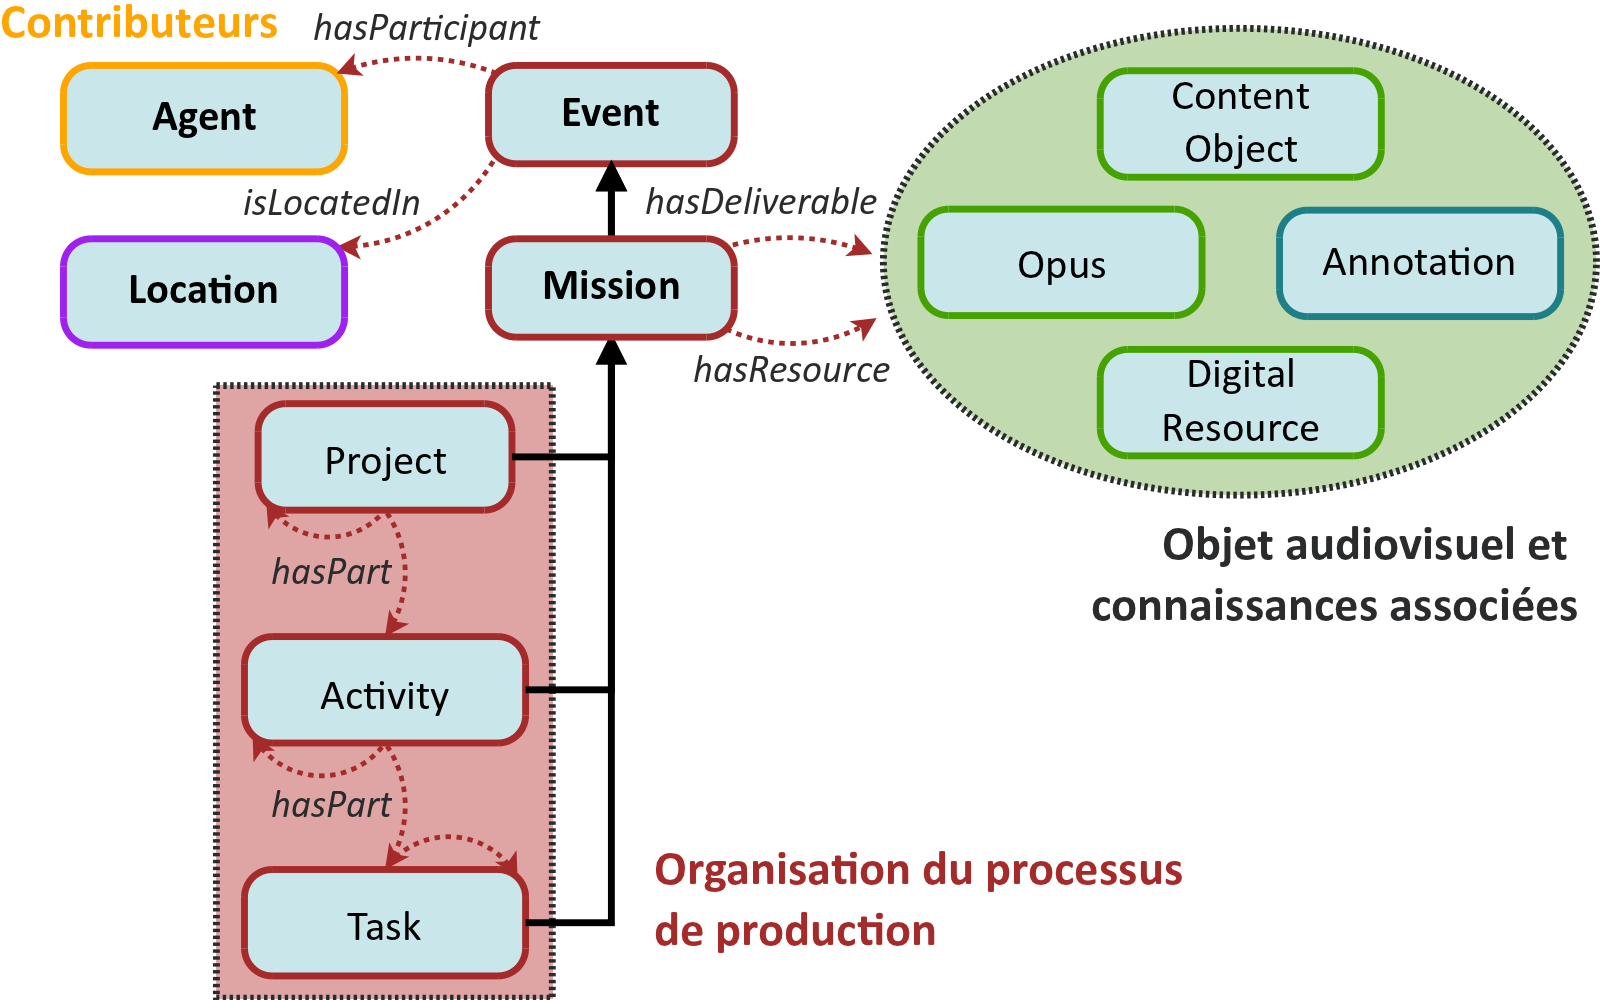
\includegraphics[width=0.75\textwidth]{./images/MOD-Process-v2.png}
\caption{Principaux concepts et relations pour modéliser une hiérarchie de tâches}
\label{img:cr-event}
\end{figure}


À cela, s'ajoute les relations qui s'appliquent spécifiquement aux \con{Mission}s : 
\begin{liste}
	\item il est possible de spécifier un ou plusieurs résultats attendus (ou livrable) pour chaque \con{Mission} (\rel{hasDeliverable}/\rel{isADeliverableOf}).
	Ce livrable peut être soit un document ou fragment audiovisuel (\con{Opus}), une séquence de matériel audiovisuel (\con{ContentObject}), un fichier (\con{DigitalResource}) ou bien une description (\con{Annotation}).
	Par exemple, une \con{Task} de tournage vise à produire une séquence audiovisuelle alors qu'une \con{Task} de transcodage vise à produire un nouveau fichier vidéo.

	\item il est possible d'associer un ou plusieurs éléments existants (ou ressource) à chaque \con{Mission} (\rel{hasResource}/\rel{isAResourceFor}). 
	Cette ressource peut être soit un document ou fragment audiovisuel (\con{Opus}), une séquence de matériel audiovisuel (\con{ContentObject}), un fichier (\con{DigitalResource}) ou bien une description (\con{Annotation}).
	Par exemple, le \con{Project} Magazine\#48 utilise des séquences audiovisuelles (\con{Segment}) tournées l'année dernière.

	\item il est possible d'indiquer un ordre de réalisation des \con{Mission}s grâce à des relations d'anteriorités (\rel{precedes}, \rel{precedesTransitive}) et de postériorités (\rel{follows}, \rel{followsTransitive}).
	Les propriétés transitives généralisent les autres propriétés afin de faciliter le raisonnement par inférence (à la manière de SKOS, \ref{sec:skos}).

	\item il est possible de spécifier des relations hiérarchiques entre les types de \con{Mission}s par la relation \rel{hasPartTransitive}/\rel{isPartOfTransitive} et \rel{hasPart}/\rel{isPartOf}.
	Nous ajoutons des restrictions afin que chaque type de Mission ne puisse englober que des Missions du même type, ou bien de niveau inférieur, de manière à créer des niveaux . 
	Ainsi, un Project peut tout englober, mais une Task ne peut s'englober qu'elle-même. 
	Inversement, une Task peut être englobée dans tous types de Mission, mais un Project ne peut qu'être englobé par lui-même.
\end{liste}





%%%%%%%%%%%%%%%%%%%%%%%%%%%%%%%%%%%%%%
\subsubsection{Les contributeurs et leur engagement dans un projet de production}\label{sec:agent}
\paragraph{Agent et compétences}
Notre modélisation des contributeurs repose sur la notion d'\con{Agent} humain ou logiciel qui possèdent des compétences (\con{Skill}) pour réaliser les \con{Mission}s qui leur sont confiées :
\begin{cadrecol}{LightGoldenrodYellow}
Un \con{Agent} représente une entité avec des capacités d'actions (contrairement à une ressource), qui peuvent être mises en oeuvre dans le cadre d'un évènement (\con{Event}).
Par exemple, l'\con{Agent} chargé d'identifier les personnes dans un plan peut être une documentaliste ou bien un logiciel de reconnaissances de visage.
\end{cadrecol}

\begin{cadrecol}{LightGoldenrodYellow}
Une \con{Skill} représente la capacité d'un contributeur à compréhendre des instructions et à réaliser la ou les actions correspondantes.
Par exemple, la compétence \gui{tournage extérieur} implique qu'un contributeur sait comment régler sa caméra, se positionner et tourner des images de bonnes qualités en lumière naturelle. 
Cela implique également qu'il connaît et comprend les instructions et les règles que l'on utilise pour un tournage à l'extérieur.
\end{cadrecol}

On distingue en particulier les compétences linguistiques, des savoir-faire professionnels : 
\begin{liste}
	\item une \con{LinguisticSkill} représente la capacité d'un contributeur à parler, lire et comprendre une langue humaine.
	\item une \con{ProfessionalSKill} représente la capacité d'un contributeur à réaliser certaines tâches liées à un domaine professionnel, ainsi qu'à comprendre les instructions et les notations utilisées dans ce domaine. 
	Par exemple, la capacité de \gui{cadrage} représente la capacité d'un contributeur à tenir une caméra en suivant les instructions de cadrage d'un réalisateur (plan large, plan rapproché etc.).
\end{liste}

\paragraph{Engagement dans un projet de production}
En plus de cette notion de contributeur, il faut également modéliser la notion d'engagement, ce qui se représente classiquement par les notions de rôle et de droits.
Dans le cadre d'une modélisation de productions audiovisuelles variées, nous devons faciliter le paramétrage des responsabilités attribuées à chacun de ces rôles. 
Pour cela, nous introduisons la notion de poste (\con{Position}), qui représente le contexte de travail d'un contributeur, et à laquelle nous rattachons des droits (\con{Right}s) sur les \con{Mission}s.

\begin{cadrecol}{LightGoldenrodYellow}
Un \con{Role} représente un poste générique d'un projet de production. 
L'attribution d'un rôle peut être soumise à la reconnaissance des compétences (\con{Skill}) du contributeur.
Par exemple, un caméraman doit avoir une compétences sur le maniement d'une caméra professionnelle.
\end{cadrecol}

\begin{cadrecol}{LightGoldenrodYellow}
Une \con{Position} représente un poste et un contexte de travail particulier.
Il s'agit de préciser quel est l'employeur du contributeur, dans quel projet de production (\con{Project}) il est impliqué ainsi que les responsabilités et les droits (\con{Right}) qu'on lui a confié. 
L'attribution d'une \con{Position} peut être soumise à la reconnaissances des compétences (\con{Skill}) du contributeur.
Par exemple, Boris est engagé en tant qu'assistant réalisateur par la RTBF dans le projet de production Magazine\#48.
Il sera chargé de réaliser les interviews hors plateau.
L'ensemble de ces informations correspond au poste de Boris.
\end{cadrecol}

Toutefois, si une \con{Position} permet de représenter les responsabilités réelles de chaque contributeur, la notion de rôle (\con{Role}), quant-à-elle, sert de repère conventionnel (auteur, réalisateur, caméraman etc.) et permet de définir des règles génériques d'attributions de droits.
Par exemple, un auteur sur un projet Z peut être responsable de l'écriture du scénario et de la continuité (ajout des dialogues et détails des actions), alors que ce travail sera confié respectivement à l'auteur et au dialoguiste sur un projet Y.
On peut également écrire une règle qui attribuent des droits de validation à un producteur sur l'ensemble du projet de production, ou juste une activité.


\paragraph{Droits et responsabilités}
Une production audiovisuelle est un projet qui se découpe en plusieurs étapes, mené à bien par des équipes de spécialistes. 
De ce fait, on attribue des droits et des responsabilités (\con{Right}) aux contributeurs (\con{HistoricalAgent}) pour une tâche ou bien une étape donnée (\con{Mission}), en fonction de son rôle et de ses compétences. 
Afin de modéliser cette relation triple (contributeur-droit-tâche), il nous faut introduire un concept intermédiaire que nous avons nommée l'ordre de mission (\con{CommissionOrder}).

\begin{cadrecol}{LightGoldenrodYellow}
Un \con{CommissionOrder} représente une délégation de droits et de responsabilités (\con{Right}) sur une \con{Mission}. 
Cette délégation s'applique à un poste (\con{Position}), et donc indirectement au contributeur (\con{HistoricalAgent}) occupant ce poste.
Par exemple, Anne est productrice et de ce fait obtient un droit de validation sur la tâche d'écriture du plan de tournage. 
\end{cadrecol}

\begin{cadrecol}{LightGoldenrodYellow}
Un \con{Right} représente le devoir et l'autorisation de réaliser un ensemble d'actions, au sens d'interdire ou d'autoriser la création, la modification, la validation ou l'accès à certaines connaissances sur un projet de production.
Par exemple, Anne (productrice) n'est pas autorisé à écrire le plan de tournage, par contre elle a le droit de le valider.
\end{cadrecol}

Nous avons défini par défaut 4 couches de droits d'accès (information, contribution, exécution et délégation) ainsi qu'un droit de validation, qui consiste à valider les résultats produits par d'autres tâches.  
Ces droits sont des exemples utilisés dans le cadre de MediaMap, d'autres types de droits peuvent être définis pour s'ajuster aux besoins de l'application visée.
Dans notre cas, chaque couche du droits d'accès rajoute de nouvelles possibilités d'actions au contributeur, de manière à ce que les couches supérieures héritent des droits des couches inférieures : 
\begin{liste}
	\item un droit d'information (\con{InformationRight}) représente un accès en lecture, un droit d'accéder aux connaissances associées à la tâche.

	\item un droit de contribution (\con{ContributionRight}) représente la possibilité de participer à la réalisation d'une tâche. 
	Il s'agit d'un droit de modification, mais pas de création, ce qui implique que la personne n'est pas responsable de l'achèvement de la tâche.

	\item une obligation de réalisation (\con{ExecutionRight}) représente la responsabilité vis-à-vis d'une tâche. 
	Il s'agit d'un droit de création et de rendu du résultat de la tâche.

	\item un droit de délégation (\con{AssignmentRight}) représente la possibilité pour un contributeur d'organiser une \con{Mission}, c'est-à-dire de créer des sous-tâches et de les déléguer à d'autres contributeurs.
	Cela correspond à un droit d'administration dans les systèmes de gestion de contenu et rajoute la possibilité de valider le résultat des sous-tâches.
\end{liste}


\begin{figure}[ht!]
\centering
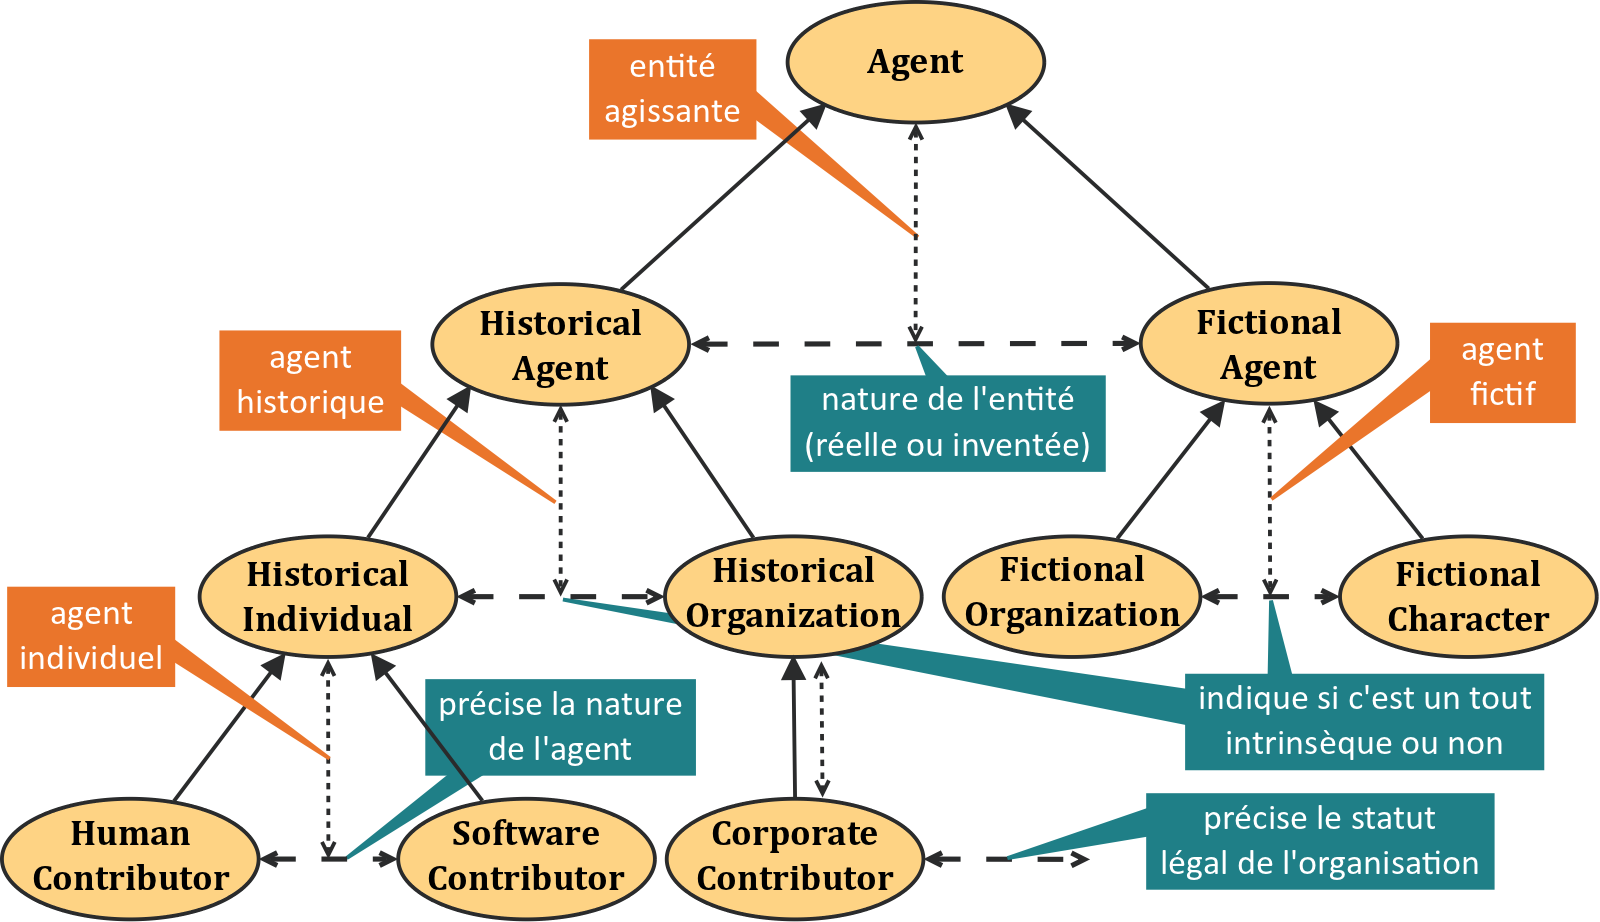
\includegraphics[width=0.95\textwidth]{./images/SO-Agent-v1.png}
\caption{Extrait de la structure ontologique qui modélise les agents et les contributeurs à un projet de production}
\label{img:so-agent}
\end{figure}

\paragraph{Structure ontologique et relations avec d'autres concepts}
La Figure \ref{img:so-agent} présente la structure ontologique concernant les différents types d'\con{Agent}s.
Le premier critère différentiel porte sur la nature réelle (\con{HistoricalAgent}) ou fictive (\con{FictionalAgent}) de l'entité agissante. 
Ensuite, nous distinguons entre les entités collectives (\con{HistoricalOrganization}, \con{FictionalOrganization}) et individuelles (\con{HistoricalIndividual}, \con{FictionalCharacter}).
Il est à noter que nous avons défini une contrainte de cohérence qui n'autorise que les \con{HistoricalAgent}s à participer à un projet de production.
Pour les organisations, nous avons défini le statut d'entreprise (\con{CorporateContributor}), qui pourrait se distinguer des associations ou autres collectifs ayant un statut légal distinct. 
Il s'agit par exemple de pouvoir représenter la RTBF, ou la VRT. 
% quid des contributeurs VS individus normaux ? 
Concernant les individus, un \con{HistoricalIndividual} permet de représenter des personnages historiques comme Churchill ou Jean Rochefort. 
À cela, nous ajoutons des spécialisations pour les contributeurs à un projet de production, qu'il s'agisse de personnes humaines (\con{HumanContributor}) ou bien d'agents logiciels (\con{SoftwareContributor}).

\begin{figure}[ht!]
\centering
\includegraphics[width=0.85\textwidth]{./images/CR-Agent&Mission-v2.png}
\caption{Principaux concepts et relations pour modéliser l'engagement des contributeurs dans un projet de production}
\label{img:cr-agent}
\end{figure}

% \paragraph{Relations avec d'autres concepts}
Concernant les relations entre ces concepts, la Figure \ref{img:cr-agent} présente une vue générale des articulations entre les contributeurs, leur engagement dans un projet de production ainsi que les droits et responsabilités qui en découlent.
Pour préciser cela, nous suivrons une lecture du diagramme à partir du coin en haut à gauche et suivant un sens de lecture gauche-droite, haut-bas.
Tout d'abord, nous précisons les relations du concept d'\con{HistoricalIndividual} :
\begin{liste}
	\item une ou plusieurs compétences (\con{Skill}) peuvent être attribué à un individu réel (\rel{hasProficiency}/\rel{isMasteredBy}).
	\item un ou plusieurs postes (\con{Position}) peuvent être attribué par un individu réel (\rel{holdsPosition}/\rel{isHeldBy}).
\end{liste}

Une fois des compétences attribués, le contributeur obtient une \con{Position} :
\begin{liste}
	\item une ou plusieurs compétences (\con{Skill}) peuvent être nécessaires pour obtenir le poste (\rel{requiresProficiency}). 
	Cette relation s'applique également à la notion de \con{Role}.
	\item le titre officiel (\con{Role}) du poste peut être précisé (\rel{worksAs}).
	\item le projet (\con{Project}) auquel le poste est rattaché peut être indiqué (\rel{withinScope}).
	\item l'organisation (\con{CorporateContributor}) qui embauche un contributeur à ce poste peut être spécifiée (\rel{worksFor}/\rel{hasWorker}).
	\item la délégation (\con{CommissionOrder}) de droits (\con{Right}) sur des tâches (\con{Mission}) peut être déclaré (\rel{grantsCommission}).
\end{liste}

Concernant les \con{CommissionOrder}, deux relations permettent de faire le lien :
\begin{liste}
	\item le détail des droits (\con{Right}) qui sont accordés (\rel{grantsRights}).
	\item la ou les tâches (\con{Mission}) pour lesquels ils sont accordés (\rel{upon}).
\end{liste}


























% \subsection{Prise en compte du multi-jargon}\label{}

% \subsubsection{Concept et termes}\label{sec:onter}
% Le modèle concept-terme que nous avons développé étend la représentation de la terminologie à son contexte d'accès, voir \cite{Diemert2010} et \cite{Diemert2011a}. Dans un premier temps, on associe à chaque concept un ou plusieurs termes, une définition voire une illustration. Chaque terme est caractérisé par son appartenance à une ou plusieurs notations qui représentent une langue, un vocabulaire métier, un code d'écriture, etc. Les fichiers peuvent être caractérisés de manière équivalente, voir figure \ref{img:mj-ct}.


% \begin{figure}[ht!]
% \centering
% 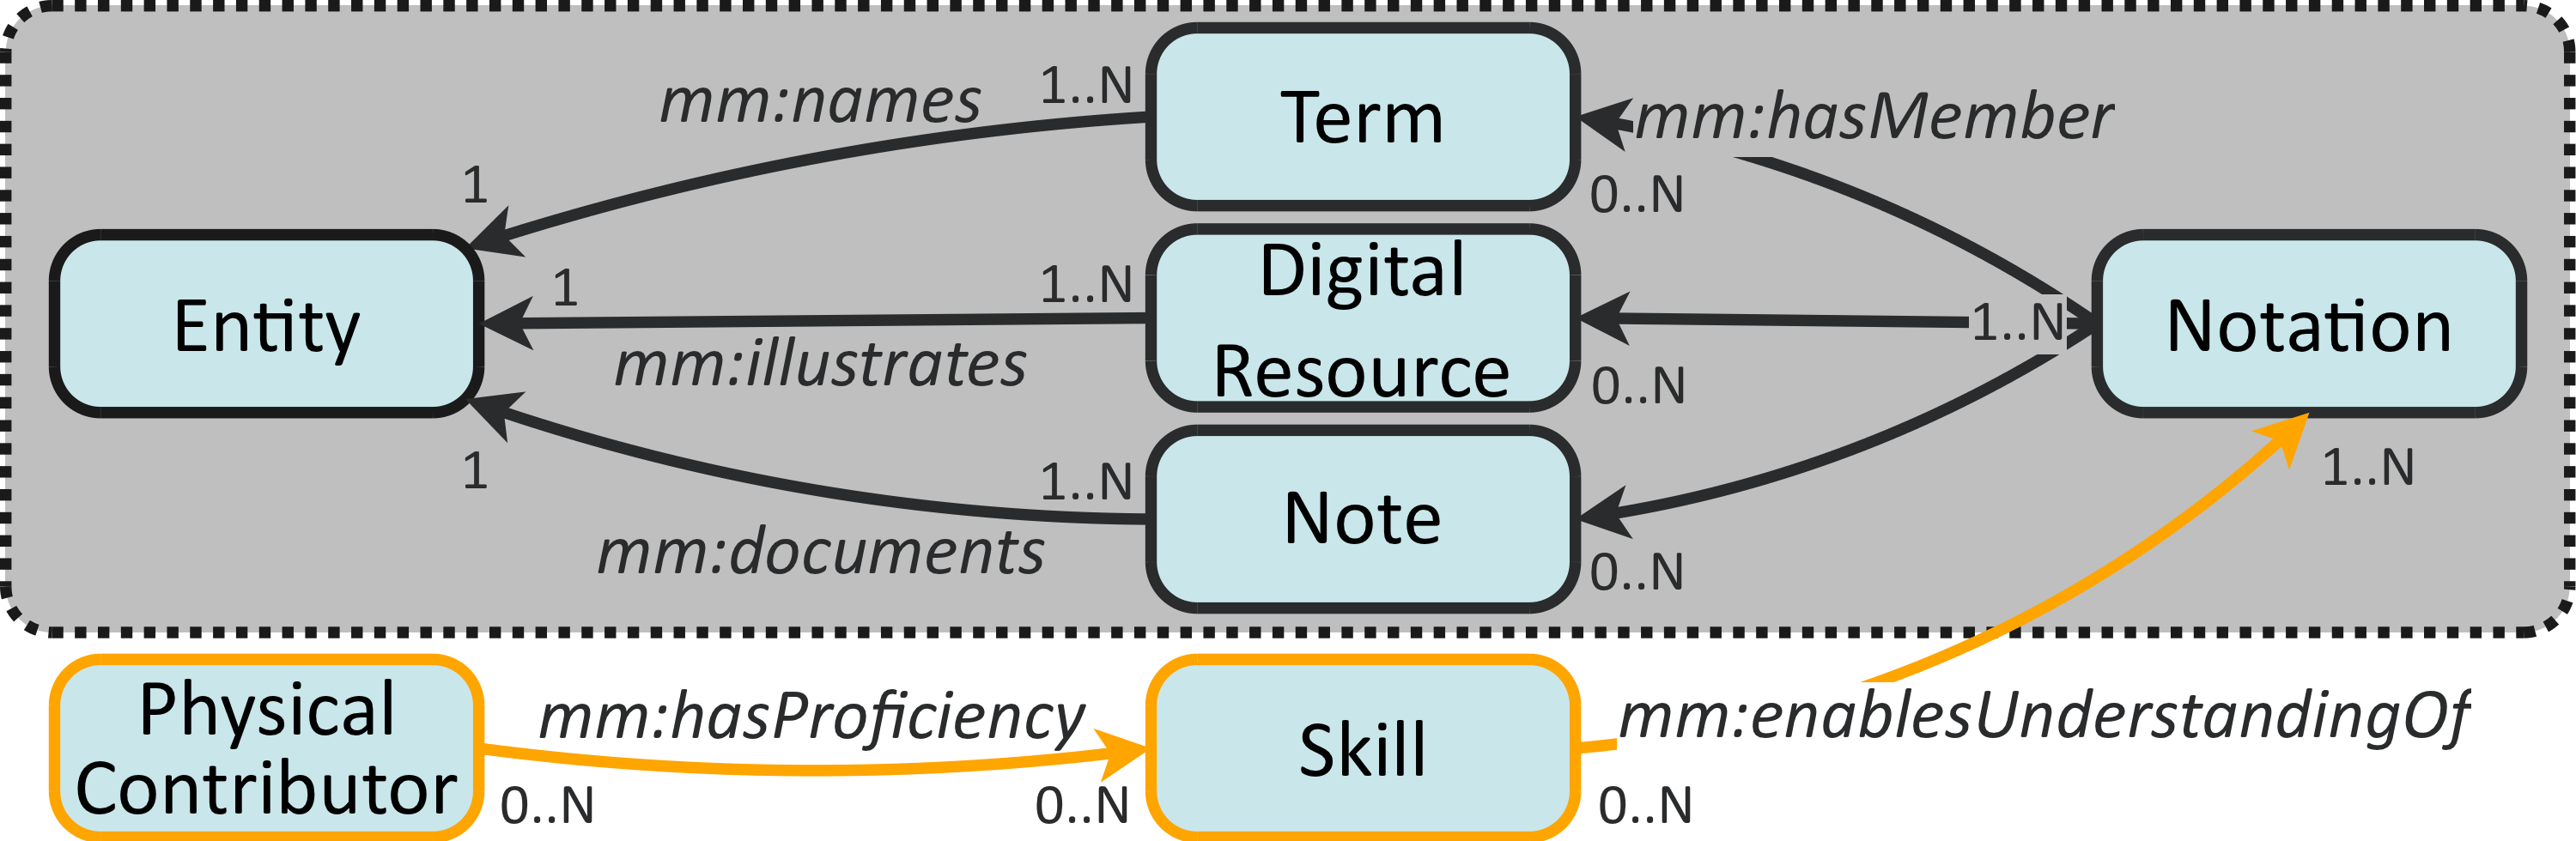
\includegraphics[width=0.75\textwidth]{./images/MOD-TermConcept-v5a.png}
% \caption{}
% \label{img:mj-ct}
% \end{figure}


% % \begin{cadrecol}{LightGoldenrodYellow}
% 	\con{Entity} représente un concept auquel on peut associer
% 		un terme (\con{Term} -- \rel{mm:names} / \rel{mm:isNamedBy}) ; une ressource média (\con{DigitalResource} -- \rel{mm:illustrates} / \rel{isIllustratedBy}) ou bien une note de documentation (\con{Note} -- \rel{mm:documents} / \rel{is\-Docu\-mentedBy}).
% % \end{cadrecol}

% % \begin{cadrecol}{LightGoldenrodYellow}
% 	\con{Term} représente un terme portant une valeur lexicale que l'on peut associer à un concept via la relation \rel{mm:names}.
% 	Un \con{Term} est caractérisé par son appartenance à un type de \con{Notation} (\rel{mm:isMemberOf} / \rel{mm:hasMember}).
% % \end{cadrecol}

% % \begin{cadrecol}{LightGoldenrodYellow}
% 	\con{Notation} représente une caractéristique commune d'un ensemble de \con{Term} ou de ressource numérique \con{DigitalResource}. 
% 	Il s'agit par exemple d'une langue, d'un format de fichier, d'un type d'encodage de date ou bien d'une structure terminologique propre à une communauté de pratiques ou une communauté d'utilisateurs.
% 	Chaque \con{Term} peut être décrit par une ou plusieurs \con{Notation}, chacune spécifiant une caractéristique particulière.
% 	Par exemple, l'étiquette \e{Plan américain} peut être décrite come appartenant à la langue française ainsi qu'à une liste d'autorité de types de plan.
% 	On distingue quatre types de \con{Notation} : 
% 	\begin{liste}
% 		\item \con{NaturalLanguage} représente les langues humaines.
% 		\item \con{SyntaxEncodingScheme} représente un codage de l'information comme l'encodage des caractères ou bien un format de fichier. 
% 		\item \con{AuthorityList} représente une liste d'autorité composé de termes. 
% 		\item \con{VocabularyEncodingScheme} (VES) représente un SOC ou un jargon propre à une organisation ou un métier.\\
% 	\end{liste}

% % \end{cadrecol}


% \paragraph{Documentation}
% % \begin{cadrecol}{LightGoldenrodYellow}
% 	\con{Note} représente une chaîne lexicale dont le but est de documenter un concept (\con{Entity}). 
% 	Nous définissons des spécialisations de \con{Note} à la manière de SKOS, par exemple pour la définition d'un concept (\con{DefinitionNote}). 
% % \end{cadrecol}

% \con{DigitalResource} représente un fichier numérique. Par exemple, un fichier texte, une photo ou bien un son. 



% \subsubsection{Conceptualisation et bases de connaissances}\label{}
% \begin{figure}[ht!]
% \centering
% 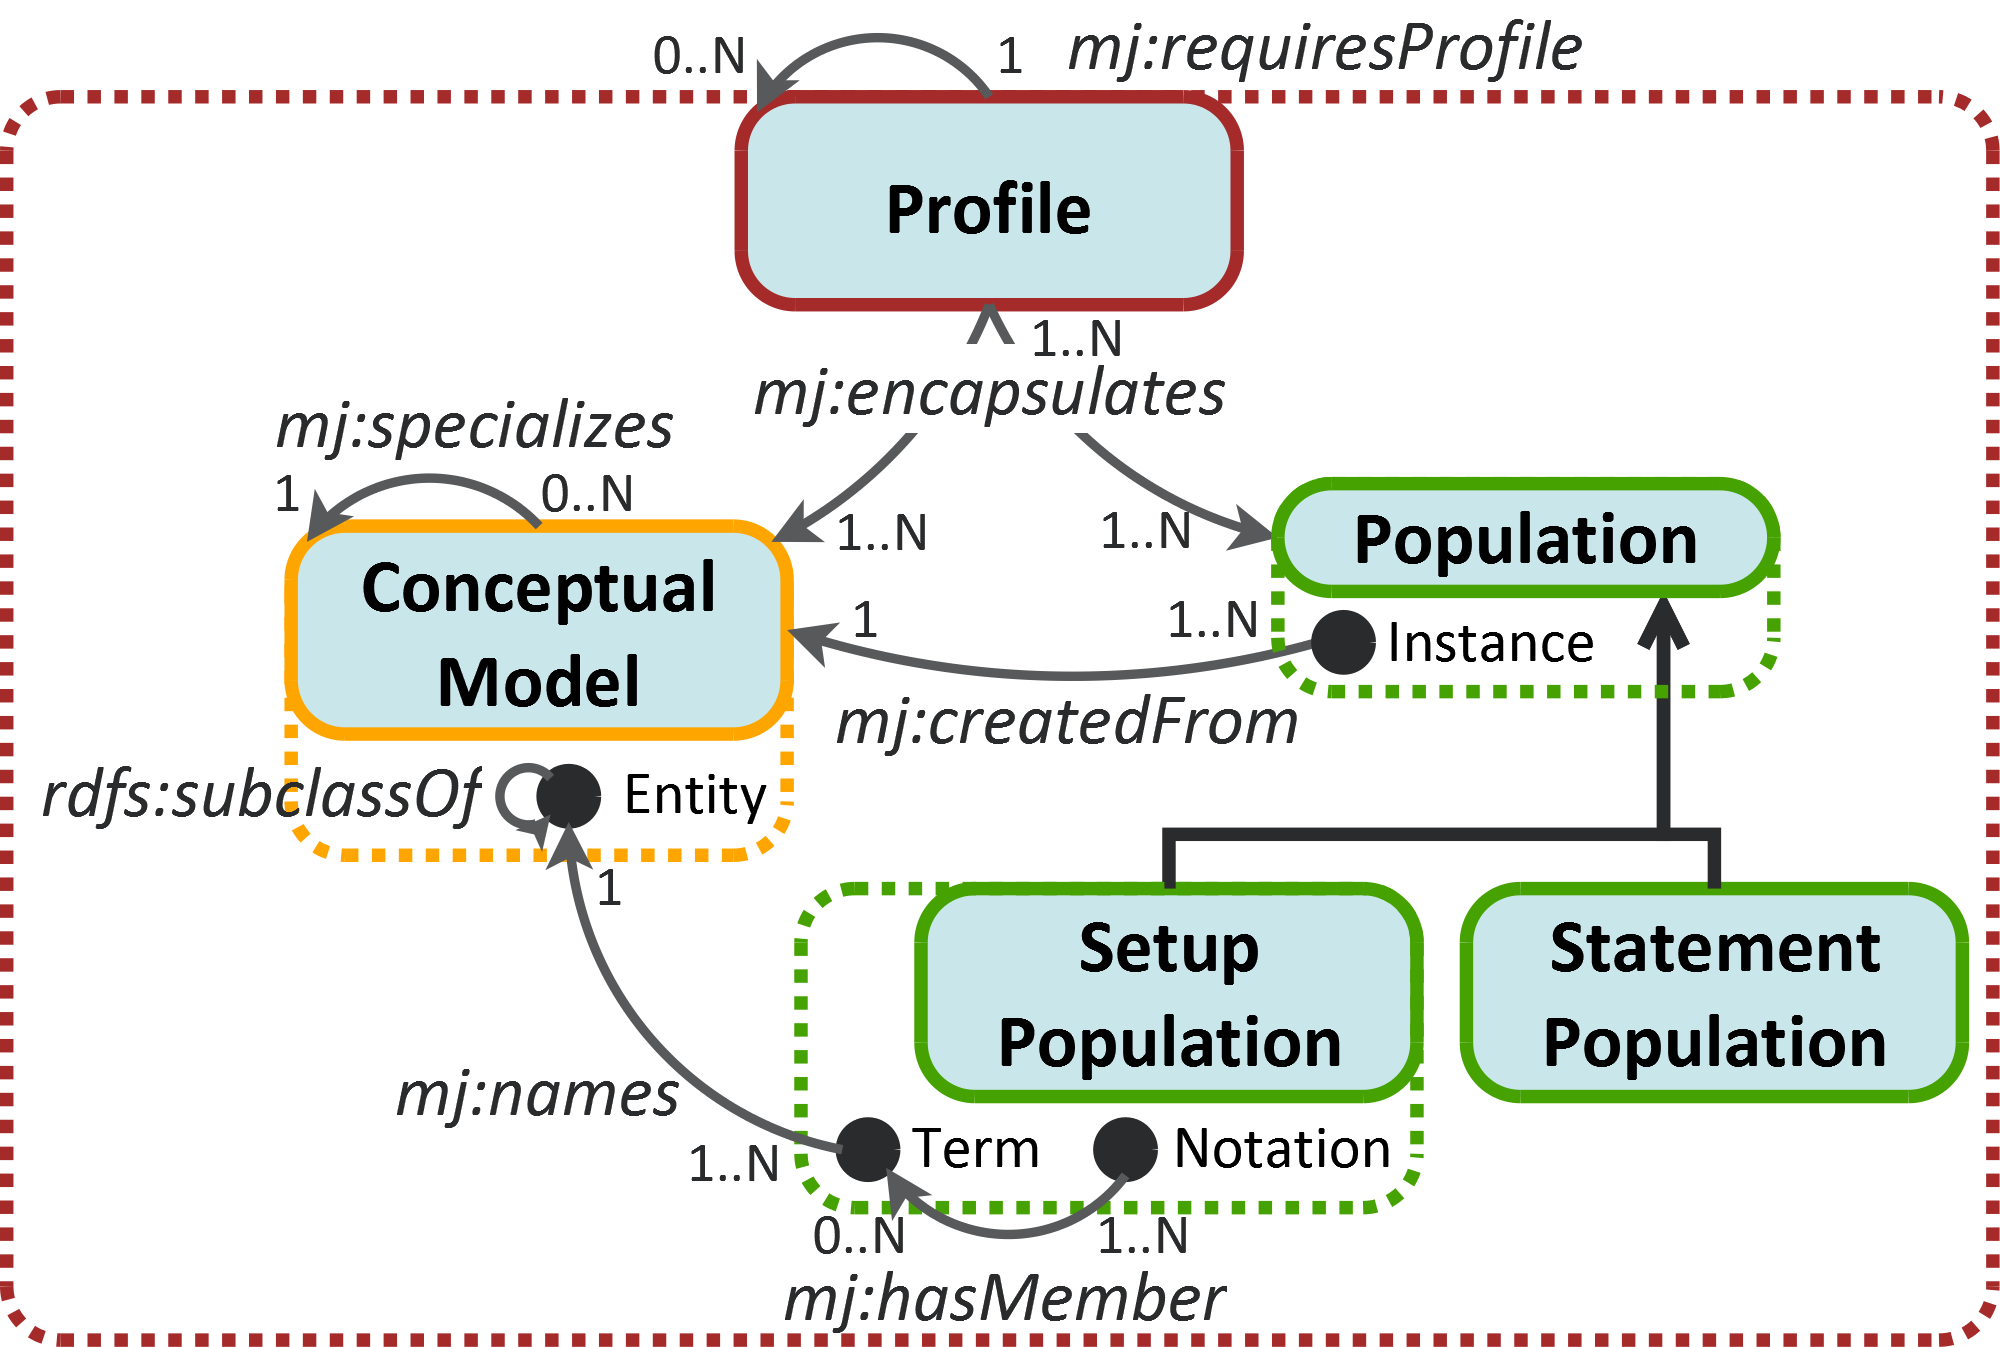
\includegraphics[width=0.7\textwidth]{./images/MOD-Profile-v3.png}
% \caption{}
% \label{img:conceptualisation}
% \end{figure}


% \subsubsection{Vue et contexte d'accès}\label{}

% % \begin{cadrecol}{LightGoldenrodYellow}
% % 	\con{} 
% % \end{cadrecol}

% \subsection{Le processus de production audiovisuelle}\label{}
% \subsubsection{Projet, Produit, Contributeur}\label{}
% \subsubsection{L'écriture filmique}\label{}


% \subsection{Le document audiovisuel}\label{}
% \subsubsection{Structure documentaire}\label{}
% \subsubsection{Manifestations}




